\documentclass{article}
\usepackage{amsmath}
\usepackage{amsthm}
\usepackage{amsfonts}
\usepackage{amssymb}
\usepackage{bbold}
\usepackage{dsfont}
\usepackage{graphicx}
\usepackage{cleveref}
\usepackage{bm}
\usepackage{booktabs}
\usepackage{siunitx}
\usepackage{xcolor}
\usepackage[utf8]{inputenc}
\usepackage[english]{babel}
\newtheorem{definition}{Definition}
\newtheorem{example}{Example}
\newcommand{\exP}[1]{\mathrm{e}^{#1}}
\newcommand{\dif}{\mathrm{d}}
\renewcommand{\vec}[1]{\mathbf{#1}}
\newcommand{\pdagger}{{\phantom{\dagger}}}
\newcommand{\state}[1]{\vert #1\rangle}
\newcommand{\cstate}[1]{\langle #1\vert}
\newcommand{\tr}[1]{\mathrm{tr}\left\{#1\right\}}
\newcommand{\trs}[2]{\, \mathrm{tr}_{#1}\{#2\}}
\newcommand{\expc}[3]{\langle #1\vert #2 \vert #3\rangle}
\usepackage[doi=false,url=false,isbn=false,backend=bibtex,style=nature,natbib=true,sorting=none]{biblatex}
\bibliography{bib.bib}
\usepackage{geometry}
\geometry{
	a4paper,
	total={170mm,257mm},
	left=20mm,
	top=20mm,
}
\begin{document}
\title{Additional results and analyses: Transport through spinfull two-site Peierls model}
\author{Rudolf Smorka}
\maketitle
%\tableofcontents
\section{Model}
\subsection{Original model}
The original two-site Peierls-model is extended by having two spin states per site
\begin{equation}
	H_\mathrm{Peierls} = \sum_{i\sigma}\varepsilon_{i\sigma}^\pdagger c_{i\sigma}^\dagger c_{i\sigma}^\pdagger + (-t_0-t_1(a^\dagger + a))\sum_\sigma (c_{1\sigma}^\dagger c_{2\sigma}^\pdagger + \mathrm{h.c.}).
\end{equation}
As is assumed in Franssons work, $\varepsilon_{i\sigma}=\varepsilon$. The formulation of the leads remains as before, except the additional spin index which distinguishes the different spin-states of the leads electrons. However, the system-lead coupling now is spin-dependent
\begin{equation}
	H_\mathrm{sys-lead} = \sum_{k_L,k_R,\sigma\sigma'} (\nu_{k_L\sigma }^\pdagger d_{k_L\sigma}^\dagger c_{1\sigma'}^\pdagger + \nu_{k_R\sigma }^\pdagger d_{k_R\sigma}^\dagger  c_{2\sigma'}^\pdagger + \mathrm{h.c.}).
\end{equation}
In the wide-band limit, the coupling matrix $\Gamma$ is then
\begin{equation}
	\Gamma_{i \sigma\sigma'}^{(L,R)} = 2\pi \sum_{k_{L,R}} \vert \nu_{k_{L,R} \sigma}\vert^2 \delta(\varepsilon_{k_{L,R}\sigma\sigma'}-\varepsilon_{i\sigma'})
\end{equation}
where $\varepsilon_{i\sigma'}$ is a system eigenenergy with spin $\sigma$. As before, we assume that $\nu_{k\sigma\sigma'} = \nu_k \delta_{\sigma\sigma'}$. 
As in the previous report, we make the classical vibration approximation, in which the Hamiltonian reads
\begin{equation}
	H_\mathrm{Peierls} = \frac{\omega_0^2 X^2}{2} + \frac{P^2}{2}  + \sum_{i\sigma } \varepsilon_i c_{i\sigma}^\dagger c_{i\sigma}^\pdagger -\left(t_0 + t_1\sqrt{2\omega_0}X\right)\sum_{\sigma}(c_{1\sigma}^\dagger c_{2\sigma}^\pdagger + \mathrm{h.c.}).
\end{equation}
\subsection{With spin-orbit coupling}
Even for the two-site system, a spin-orbit coupling term can be introduced. The Peierls-Hamiltonian with this SOC then reads
\begin{equation}
	H_\mathrm{Peierls+SOC} = H_\mathrm{Peierls} + \sum_{m,n=1}^2( c_{m\uparrow}^\dagger W_{m,n}^\pdagger c_{n\downarrow}^\pdagger + c_{m\downarrow}^\dagger W^\times_{m,n} c_{n\uparrow}^\pdagger).
\end{equation}
In the following, we assume the diagonal elements to be $W_{n,n}=\alpha_n$ and the off-diagonal to be $W_{n,m} = \beta$ ($n\neq m$). 
A minimal model has been proposed in \cite{Gutierrez_Díaz_Naaman_Cuniberti_2012}, where $W^\times_{n,n} = (W_{n,n})^*$ and $W_{n,n+1}^\times = -(W_{m,n})^*$ so that the Hamiltonian is hermitian. 
\section{Parameters}
To simplify the analysis, we assume $\varepsilon_i = \varepsilon_j = \varepsilon_0$, and set the parameters to
\begin{align*}
	\varepsilon_0 &= \SI{0}{\milli\electronvolt}\\
	\omega_0 &= \SI{0.1}{\electronvolt}\\
	t_0 &= \SI{2}{\electronvolt}\\
	t_1 &= \SI{0.2}{\electronvolt}\\
	\Gamma &= \SI{10}{\milli\electronvolt}\\
	T &= \SI{5}{\milli\electronvolt}.
\end{align*}
These are the same as in the previous report. We assume that the SOC parameters $\alpha,\beta$ are free. 
For the parameters used in \cite{Gutierrez_Díaz_Naaman_Cuniberti_2012} (with an estimated SOC paramater $\alpha=\SI{2}{\milli\electronvolt \nano\meter}$), they are  $\alpha_0 = (0.423-0.307i) \SI{}{\milli\electronvolt}$, $\alpha_1 = (-0.157-0.095i)\SI{}{\milli\electronvolt}$ and $\beta = (0.783-0.276i)\SI{}{\milli\electronvolt}$. What is strange in their approach, when I generalize the functions $\Psi(z)$ and $f(z) = \partial_z \Psi(z)$ to multiple sites, then the diagonal elements are increasing with increasing size of the system (way beyond $\sim\SI{1}{\electronvolt}$).
 %, where the coupling matrix $W$ has following elements
%\begin{align}
%	W_{nn} &= -\alpha f(n\Delta z)\\
%	W_{n,n+1} &= \frac{\alpha}{2\Delta z}\Psi(n\Delta z)\\
%	W_{n,m}^\times &= -(W_{m,n})^*\\
%	W_{n,n}^\times &= (W_{n,n})^*\\
%	f(z) &= \partial_z \Psi(z)\\
%	\Psi(z) &= \sum_{l=-1/2}^{1/2}\sum_{j=1}^2 \exP{-iQ j\Delta z} g_{l,j}(z)\\
%	Q &=\frac{2\pi}{b}\\	
%	g_{l,j}(z) &= \frac{1}{\sqrt{\left(1+\left[\frac{z-lb-j\Delta z}{a}\right]^2\right)^3}}.
%\end{align}
%Here, $\alpha=\hbar \lambda E_0$ is the spin-orbit coupling parameter, $\lambda = \frac{e\hbar}{(2mc)^2}$ the SOC strength, $E_0$ the local field of the charge distribution, $b$ is the helix pitch and $a$ the helix radius. The authors use $\alpha = \SI{5}{\milli\electronvolt \nano\meter}$.
\section{Diagonalization within single-particle subspace}
\subsection{Peierls model}
Within the single-particle sub-space, the eigenstates and eigenvalues of the original Peierls model are 
\begin{align}
	\vert \psi_{\pm \uparrow}\rangle &= \frac{1}{\sqrt{2}}\begin{pmatrix}
		\pm 1 \\
		0 \\
		1 \\
		0
	\end{pmatrix} & \varepsilon_{\pm \uparrow,\downarrow} = \varepsilon\pm \vert t_0+t_1\sqrt{2\omega}X\vert\\
	\vert \psi_{\pm \downarrow}\rangle &= \frac{1}{\sqrt{2}}\begin{pmatrix}
		0 \\
		\pm 1 \\
		0 \\
		1
	\end{pmatrix} & .
\end{align}
They are spin-degenerate, since in the original model all couplings are the same for both $\sigma=\uparrow,\downarrow$. In this basis the electron-vibrational Hamiltonian is 
\begin{equation}
	\tilde{H}_\mathrm{el-vib} = -(t_0 + t_1\sqrt{2\omega}X)\begin{pmatrix}
		1 & 0 & 0 & 0\\
		0 & 1 & 0 & 0\\
		0 & 0 & -1 & 0\\
		0 & 0 & 0 & -1\\
	\end{pmatrix}
\end{equation} 
where we used the ordering $\vert \psi_{-\uparrow}\rangle, \vert \psi_{-\downarrow}\rangle, \vert \psi_{+\uparrow}\rangle, \vert \psi_{+\downarrow}\rangle$. 
The system-lead coupling is now depending on the spin polarization $P$ of the lead
\begin{equation}
	\Gamma_L = \gamma_L (1+P\sigma^z_1) = \gamma_L \begin{pmatrix}
	1+p & 0 & 0 & 0\\
	0 & 1-p & 0 & 0\\
	0 & 0 & 0 & 0\\
	0 & 0 & 0 & 0
	\end{pmatrix}
\end{equation}
introducing $p=\frac{P}{2}$. The coupling to the right lead $\Gamma_R$ is spin-independent and couples to the right site only
\begin{equation}
	\Gamma_R= \begin{pmatrix}
		0 & 0 & 0 & 0\\
		0 & 0 & 0 & 0\\
		0 & 0 & \gamma_R & 0\\
		0 & 0 & 0 & \gamma_R	
	\end{pmatrix}
\end{equation}
The coupling matrices in the single-particle eigenstate basis are
\begin{align}
	\tilde{\Gamma}_L &= \frac{\gamma_L}{2}\begin{pmatrix}
		1+p & 0 & -1-p & 0 \\
		0 & 1-p & 0 & -1+p \\
		-1-p & 0 & 1+p & 0 \\
		0 & -1+p & 0 & 1-p 
	\end{pmatrix},\\
	\tilde{\Gamma}_R &= \frac{\gamma_R}{2}\begin{pmatrix}
		1 & 0 & 1 & 0\\
		0 & 1 & 0 & 1\\
		1 & 0 & 1 & 0\\
		0 & 1 & 0 & 1
	\end{pmatrix}
\end{align}
\begin{figure}[!h]
	\centering
	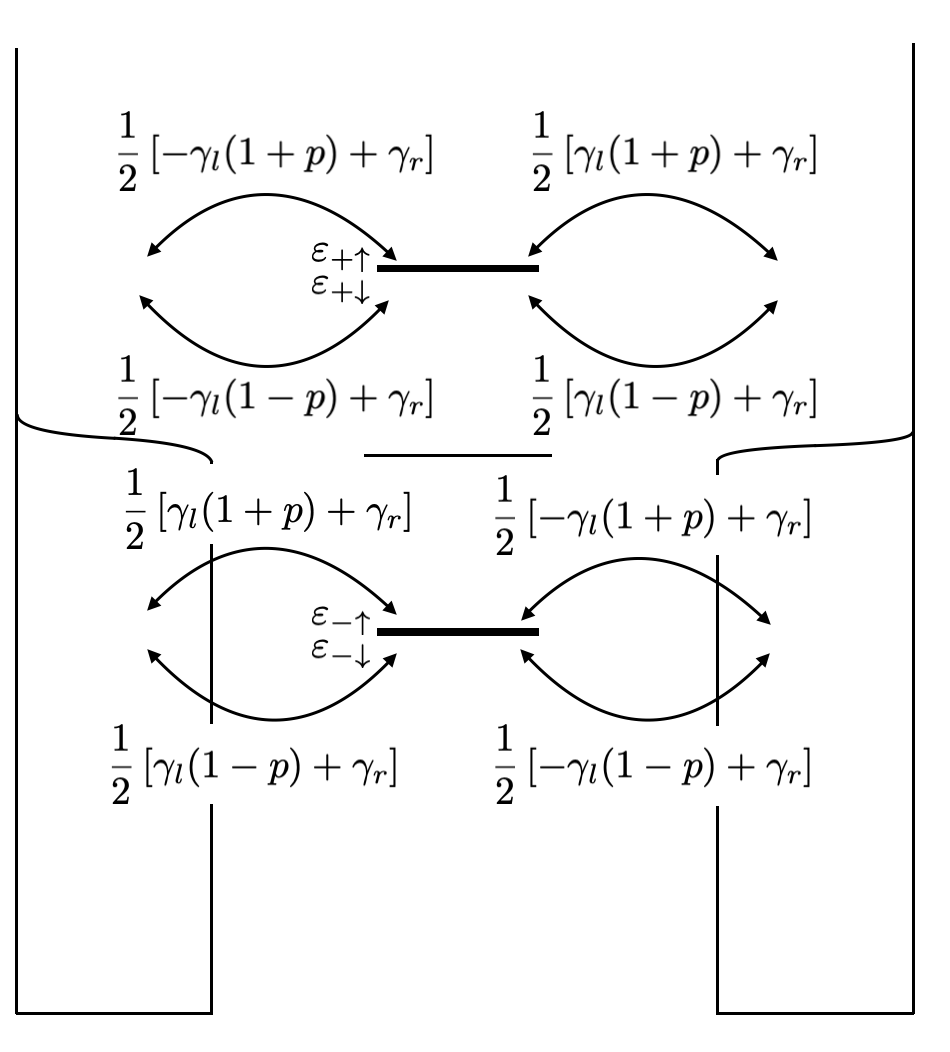
\includegraphics[width=0.4\textwidth]{figs/diagonalized_coupling.png}
	\caption{Schematic of the two-site spinfull Peierls model coupled to two leads in the single-particle eigenbasis of the uncoupled Hamiltonian with system-lead couplings in this basis.}
\end{figure}
The influence of a spin-dependent molecule-lead coupling can be seen from diagonalizing the effective Hamiltonian
\begin{equation}
	H_\mathrm{eff} = \begin{pmatrix}
		\varepsilon - i\gamma_l\left(1+\frac{P}{2}\right) & 0 & \xi & 0\\
		0 & \varepsilon - i\gamma_l\left(1-\frac{P}{2}\right) & 0 & \xi\\
		\xi & 0 & \varepsilon - i\gamma_r & 0\\
		0 & \xi & 0 & \varepsilon - i\gamma_r
	\end{pmatrix}
\end{equation}
\subsection{Peierls + SOC}
\section{Exact diagonalization of the interacting molecule}
\section{Mean-field potential}
\subsection{Peierls}
\subsection{Peierls+SOC}
\end{document}




